\section{Netzwerkklassen} \label{sec:graph_classes}

Netzwerkklassen sind eine Sammlung von Netzwerken, die bestimmte Eigenschaften teilen.
Diese Eigenschaften können z. B. die Zahl der Knoten, die Anzahl Kanten oder die topologischen Indizes sein.
Brandstädt et al. und später Bang-Jensen et al. sowie Emmert-Streib et al. fassen populäre Graph-Modelle respektive Graphenklassen in verschiedenen Werken zusammen \cite{brandstadt_graph_1999,bang-jensen_basic_2018,emmert-streib_mathematical_2020}.
In den nachfolgenden Abschnitten folgen die bedeutendsten Netzwerkklassen nach \cite{emmert-streib_mathematical_2020}.
Sie bilden die Grundlage für die Weiterarbeit in der Thesis und werden vor allem in der Datenaufbereitung und den Experimenten verwendet.

Nachfolgend werden die Eigenschaften der unterschiedlichen Netzwerkklassen \enquote{Random}, \enquote{Small World} und \enquote{Scale-free} miteinander verglichen.
Dabei werden die Struktur, die Verteilung der existierenden Grade und die Adjazenzmatrix visualisiert und beschrieben.
Zur Einführung sind reguläre, zufällige und Small-World-Graphen auf Abbildung \ref{fig:random_scale_small} visualisiert.

\begin{figure}[H]
    \centering
    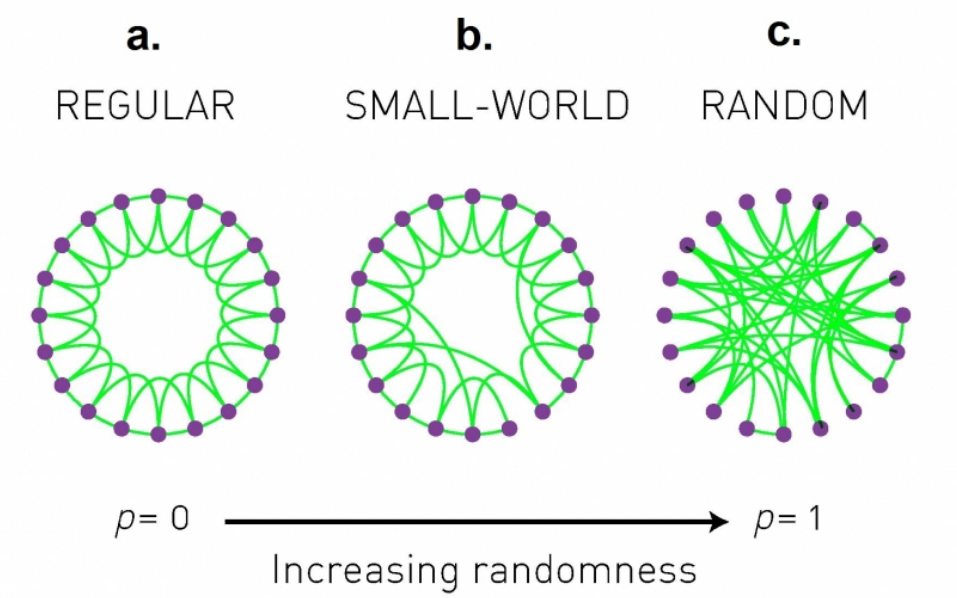
\includegraphics[width=7cm]{images/20_material_methods/barabasi_zusammenhang_smallworld_random.png}
    \caption{Eigenschaften der unterschiedlichen Netzwerkklassen (Quelle: Barabási \cite[p.~97]{barabasi_network_2016})}
    \label{fig:random_scale_small}
\end{figure}

\newpage
\subsection{Random}

Ein Zufallsgraph (engl. random graph) ist ein Graph, der zufällig gemäss einer Wahrscheinlichkeitsverteilung über die Menge aller möglichen Graphen generiert wird.
Das Studium von Zufallsgraphen ist ein Zweig der Graphentheorie und der probabilistischen Kombinatorik.

Ein gängiges Modell zum Erzeugen eines Zufallsgraphen ist das Erdős-Rényi-Modell, bei dem jede mögliche Kante unabhängig mit einer festen Wahrscheinlichkeit $p$ aufgenommen wird \cite[p.~205 ff]{grimmett_random_nodate}.
Dieses Modell ist umfassend untersucht und weist besonders interessante Eigenschaften auf wie den Phasenübergang, der bei der kritischen Wahrscheinlichkeit $p = 1/n$ auftritt, wobei $n$ die Anzahl der Scheitelpunkte im Graphen ist \cite[p.~152]{bollobas_random_2001}.

Des Weiteren ist das bevorzugte Bindungsmodell (engl. preferential attachment) zu nennen, das einen Zufallsgraphen erzeugt, indem es mit einer kleinen Anzahl von Scheitelpunkten beginnt und nacheinander neue Scheitelpunkte hinzufügt, von denen jeder mit einer bestimmten Wahrscheinlichkeit proportional mit vorhandenen Scheitelpunkten verbunden ist \cite[p.~2f]{albert_diameter_1999}.
Dieses Modell wird häufig verwendet, um das Wachstum von sozialen Netzwerken oder des World Wide Web (WWW) zu modellieren.
Es gibt zahlreiche andere Modelle zum Generieren von Zufallsgraphen, jedes hat seine einzigartigen Eigenschaften. Einige Beispiele sind das Small-World, das Watts-Strogatz und das k-reguläre Modell \cite[p.~398f.]{newman_networks_2010}.

Das Studium von Zufallsgraphen hat zu einem tieferen Verständnis der Struktur und Eigenschaften realer Graphen sowie zur Entwicklung effizienter Algorithmen zum Generieren und Analysieren grosser Graphen geführt.
Auf Abbildung \ref{fig:random_graphs} sind drei Zufallsgraphen ersichtlich; gewisse Knoten besitzen einen Grad $k = 0$, was bedeutet, dass sie isoliert sind und keine Kanten haben \cite[p.~85]{barabasi_network_2016}:

\begin{figure}[H]
    \centering
    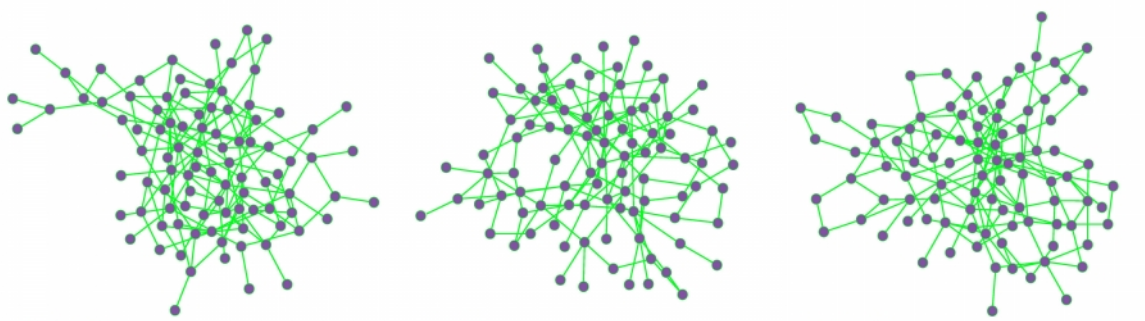
\includegraphics[width=11cm]{images/20_material_methods/random_graphs.png}
    \caption{Drei Random-Graphen mit $\protect p = 0.03$ und $\protect N = 100 $ (Quelle: Barabási. \cite[p.~84]{barabasi_network_2016})}
    \label{fig:random_graphs}
\end{figure}

\newpage
\subsection{Small World}

Ein Small-World-Graph ist eine Art komplexes Netzwerk, das sowohl eine hohe Clusterbildung als auch eine kurze durchschnittliche Pfadlänge aufweist.
Das Konzept der Small-World-Graphen ist erstmals in den 1960er-Jahren von Stanley Milgram durch das \enquote{Six Degrees of Separation}-Experiment eingeführt worden.
Er hat gezeigt, dass zwei beliebige Menschen auf der Erde durchschnittlich über sechs Bekanntschaften verbunden sind  \cite[p.~62]{travers_experimental_1969}

Ende der 1990er-Jahre haben Duncan J. Watts und Steven H. Strogatz das Konzept der Small-World-Graphen weiterentwickelt und den Begriff \enquote{Small-World Networks} eingeführt \cite[p.~440]{watts_collective_1998}.
Sie haben damit gezeigt, dass Small-World-Netzwerke durch eine hohe Clusterbildung gekennzeichnet sind, was bedeutet, dass Knoten in der Regel mit anderen Knoten zusammenhängen, die wiederum eng mit diesen verbunden sind, genauer gesagt durch eine kurze durchschnittliche Pfadlänge.
Dies heisst, dass es unkompliziert ist, jeden Knoten im Netzwerk durch eine vergleichsweise kleine Anzahl von Schritten zu erreichen.

Watts und Strogatz (1998) definieren in ihrem Modell zum Aufbau von Small-World Networks $n$ Knoten, wobei jeder Knoten mit $m$ nächsten Nachbarn verbunden ist.
Dies wird als reguläres Gitter bezeichnet (siehe Abbildung \ref{fig:small_world}), wobei $n = 10$ und $m = 4$ ist  \cite{gayen_small_2020}.
\begin{figure}[H]
    \centering
    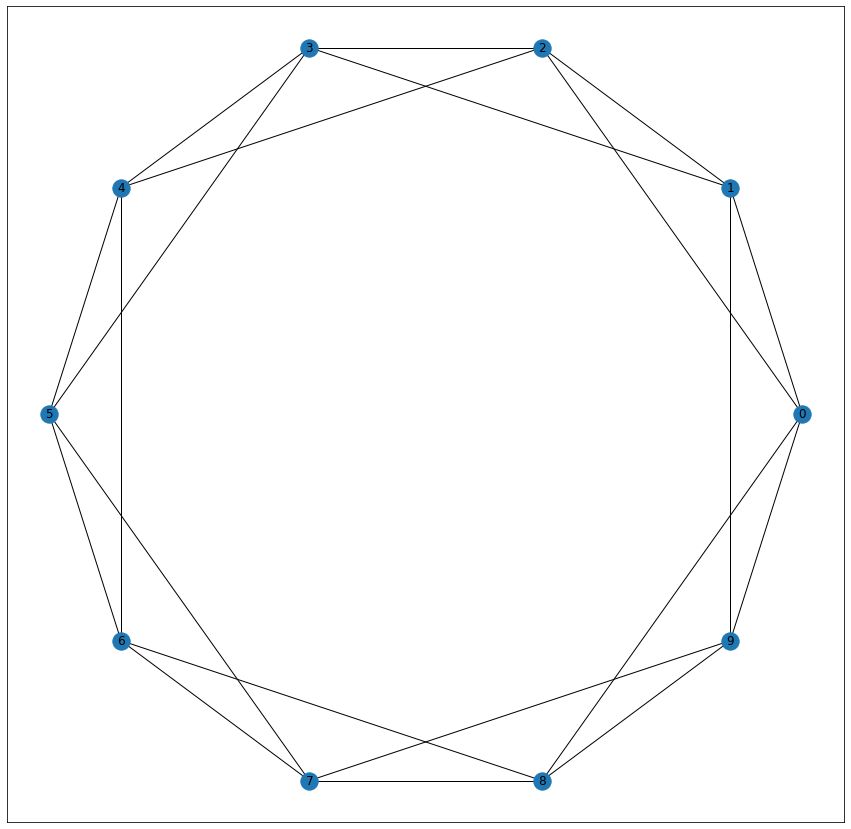
\includegraphics[width=3cm]{images/20_material_methods/small_world_lattice.png}
    \caption{Regular Lattice Graph (Quelle: Gayen \cite{gayen_small_2020})}
    \label{fig:small_world}
\end{figure}
Bei Betrachtung einer jeden Kante $(u, v)$ wird mit der Wahrscheinlichkeit $p$ zufällig ein Knoten $w$ ausgewählt und die Kante $(u, v)$ so verbunden, dass sie zu $(u, w)$ wird.
Für $p = 0$ behält es seine Struktur und hat einen hohen durchschnittlichen Abstand und eine hohe Clusterbildung.
Für $p = 1$ wird ein Zufallsnetzwerk mit kleiner durchschnittlicher Distanz und geringer Clusterbildung gebildet \ref{fig:small_world_lattice_n10}, wobei $n = 10$, $m = 4$ und $p = 1$ ist.
Für einen Zwischenwert von $p$ erhält man ein ideales Small-World Network mit geringer durchschnittlicher Entfernung und hoher Clusterbildung \cite{gayen_small_2020}.
\begin{figure}[H]
    \centering
    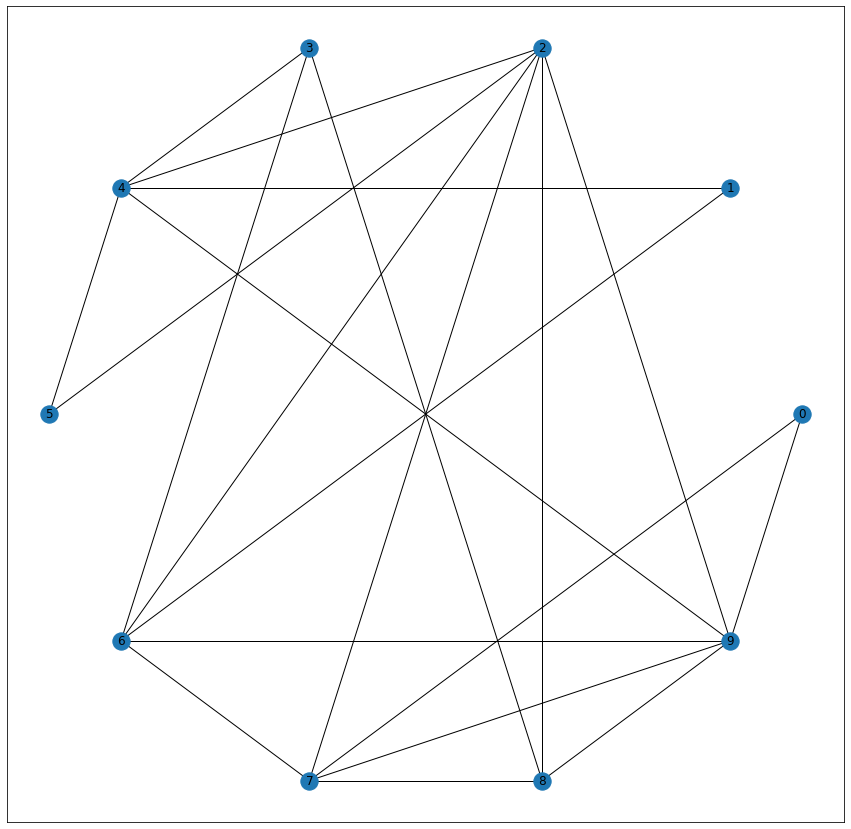
\includegraphics[width=3cm]{images/20_material_methods/small_world_lattice_n10.png}
    \caption{Regular Lattice Graph mit $n = 10, m = 4$ und $p = 1 $ (Quelle: Gayen \cite{gayen_small_2020})}
    \label{fig:small_world_lattice_n10}
\end{figure}
Es hat sich herausgestellt, dass Small-World-Graphen in Systemen der realen Welt weitverbreitet sind, darunter soziale Netzwerke, Transportnetzwerke und das Internet \cite[p.~4]{barabasi_emergence_1999}.
Sie werden auch in verschiedenen Bereichen wie Physik, Biologie und Informatik untersucht, da sie bedeutende Auswirkungen auf die Verbreitung von Informationen und die Robustheit von Netzwerken haben \cite[p.~2]{newman_structure_2003}.

\subsection{Scale-free}

In der Anfangsphase des Web, in den 1990er-Jahren, wurde davon ausgegangen, dass dieses die Eigenschaften eines zufälligen Netzwerks hat, des Netzwerktyps, der von Erdős–Rényi (1960) mathematisch charakterisiert wurde und in dem die Wahrscheinlichkeit für die Verbindung zweier Knoten als Konstante angegeben ist.
In einem derartigen Netzwerk folgt die Gradverteilung der Poisson-Form \cite{barabasi_network_2016}.

Albert et al. (1999, S. 1) haben gezeigt, dass das WWW nicht diese zufällige Netzwerkstruktur hat \cite{albert_diameter_1999}.
Tatsächlich ist die Gradverteilung ein Potenzgesetz, bei dem die Wahrscheinlichkeit, dass ein Knoten den Grad $k$ hat, proportional zu $k-\lambda$ ist, wobei $\lambda$ etwa $2$ ist.
Ein solches Netzwerk hat andere Eigenschaften, als ein zufälliges Netzwerk, da ein Potenzgesetz weniger stark abfällt als eine Poisson-Kurve.
Anstatt dass praktisch alle Knoten mehr oder weniger den gleichen Grad haben, sind einige wenige Knoten äusserst stark verbunden und die überwiegende Mehrheit hat einen geringeren Grad als der Durchschnitt \cite{barabasi_network_2016}.

\subsection{Bäume}

Ein Baum (engl. Tree) ist ein gerichteter Graph, der keine Schleifen und Kreise enthält.
Das bedeutet, dass jeder Knoten genau einen Vorgänger hat und dass es einen eindeutigen Pfad von jedem Knoten zum Wurzelknoten gibt \cite{cayley_analytical_1881}.

Die Verwendung von Bäumen ist eine gängige Methode zur Simulation von Hierarchien und Untersuchung von Struktureigenschaften in komplexen Netzwerken.
Zum Beispiel kann ein Baum Graph verwendet werden, um die Verteilung von Informationsflüssen in einem Netzwerk zu untersuchen oder um die Effekte von Strukturänderungen auf die Effizienz von Netzwerken zu bewerten \cite{brandstadt_graph_1999}.

Ein weiterer Vorteil von Baum Graphen ist, dass sie einfach zu generieren sind und wenig Rechenaufwand erfordern.
Daher sind sie für Anwendungen zweckmässig, bei denen schnelle und einfache Simulationen erforderlich sind, insbesondere bei der Analyse von grossen Netzwerken. Zudem können Baum Graphen auch verwendet werden, um statistische Eigenschaften komplexer Netzwerke zu schätzen, etwa die Verteilung von Knotengrössen oder die Anzahl der Verbindungen zwischen Knoten.

Insgesamt bieten Baum Graphen eine geeignete Methode zur Analyse von Hierarchien und Strukturen in komplexen Netzwerken.
Sie benötigen wenig Rechenaufwand und bieten relevante Informationen über die Eigenschaften von Netzwerken.
Daher sind sie ein wesentlicher Bestandteil der Netzwerktheorie und werden oft in der Praxis verwendet \cite{cayley_analytical_1881,emmert-streib_mathematical_2020}.

\begin{figure}[H]
    \centering
    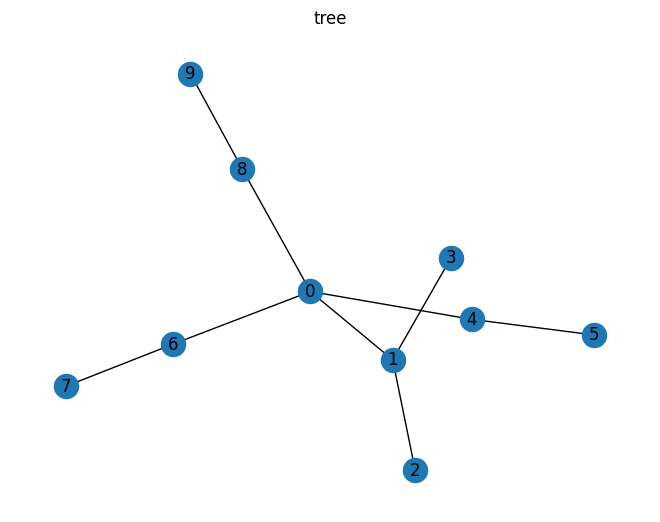
\includegraphics[width=6cm]{images/20_material_methods/tree.png}
    \caption{Baum Graph}
    \label{fig:tree-graph}
\end{figure}

\subsubsection{Sterne}

Sterngraphen sind eine Klasse von ungerichteten Graphen und eine Unterklasse von Bäumen, bei denen ein Knoten (zentraler Knoten) direkt mit allen anderen Knoten (Peripherie-Knoten) verbunden ist. 
Ein Sterngraph mit $n$ Knoten kann als $S_n$ dargestellt werden. 
Der zentrale Knoten in einem Sterngraphen hat $n-1$ Kanten, während jeder Peripherie-Knoten nur eine Kante hat.

Die Formel für die Anzahl der Kanten eines Sterngraphen lautet:
\begin{equation}
    \text{E}(S_n) = n-1
\end{equation}
Sterngraphen haben folgende Eigenschaften:
\begin{enumerate}
    \item Sie besitzen $n$ Knoten und $n-1$ Kanten.
    \item Sie haben keine Schleifen.
    \item Ihr Durchmesser ist $\min{2, n}$.
    \item Sie sind zusammenhängend.
\end{enumerate}

Sie sind einfach zu konstruieren und zu analysieren und werden oft verwendet, um Probleme in verschiedenen Bereichen zu lösen.

\begin{figure}[H]
    \centering
    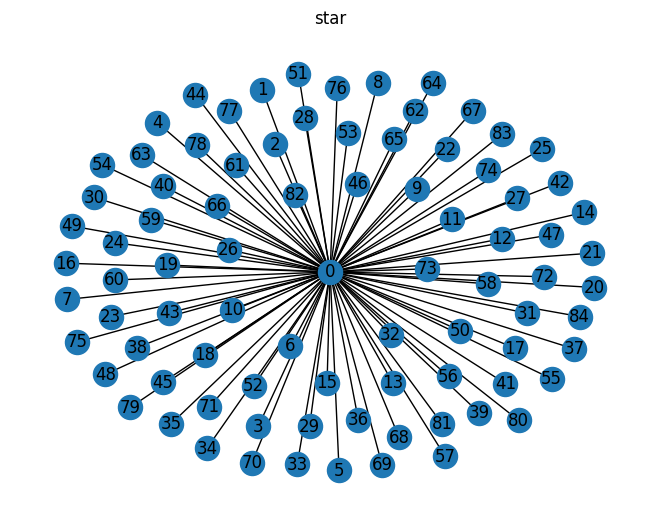
\includegraphics[width=6cm]{images/20_material_methods/star.png}
    \caption{Sterngraph}
    \label{fig:star-graph}
\end{figure}

\subsection{Vollständig} \label{sec:complete}

Vollständige Graphen sind eine bedeutsame Klasse von Graphen in der Mathematik, die eine vollständige Verbindung aller Knoten innerhalb des Graphen darstellen.
Bei einem vollständigen Graphen mit $n$ Knoten ist jeder Knoten mit jedem anderen direkt verbunden.
Ein vollständiger Graph mit $n$ Knoten kann als $G(n)$ dargestellt werden.

Die Formel für die Anzahl der Kanten eines vollständigen Graphen lautet \cite[p.~53]{barabasi_network_2016}:
\begin{equation}
    \text{E}(G(n)) = \frac{n(n-1)}{2}
\end{equation}

Ein Complete Graph ist ein besonderer Fall des k-regulären Graphen, bei dem jeder Knoten eine gleichmässige Anzahl von Kanten hat.
Er ist der maximale k-reguläre Graph für $k = n-1$ \cite{bang-jensen_basic_2018}.

\begin{figure}[H]
    \centering
    \includesvg[width=4cm]{images/20_material_methods/k5-graph.svg}
    \caption{K5-Graph}
    \label{fig:k5-graph}
\end{figure}

\subsection{Path}

Path Graphs, auch bekannt als Pfadgraphen, sind eine einfache Klasse von Graphen, die eine gerichtete Kette von Knoten darstellen.
Ein Path Graph mit $n$ Knoten kann als $P_n$ dargestellt werden.
Jeder Knoten in einem Pfadgraphen hat genau eine eingehende und eine ausgehende Kante, ausser dem ersten Knoten, der nur eine ausgehende, und dem letzten Knoten, der nur eine eingehende Kante hat.

Die Formel für die Anzahl der Kanten eines Path Graph lautet:
\begin{equation}
    \text{E}(P_n) = n-1
\end{equation}

Path Graphs finden häufig Anwendung in der Mathematik, insbesondere bei der Untersuchung von Problemen in der Graphtheorie und Netzwerktheorie \cite{bender_lists_2010}. 
Zum Beispiel können Path Graphs verwendet werden, um den kürzesten Pfad in einem Netzwerk zu untersuchen, und sie können auch als Bausteine für die Konstruktion von grösseren Graphen verwendet werden.

\begin{figure}[H]
    \centering
    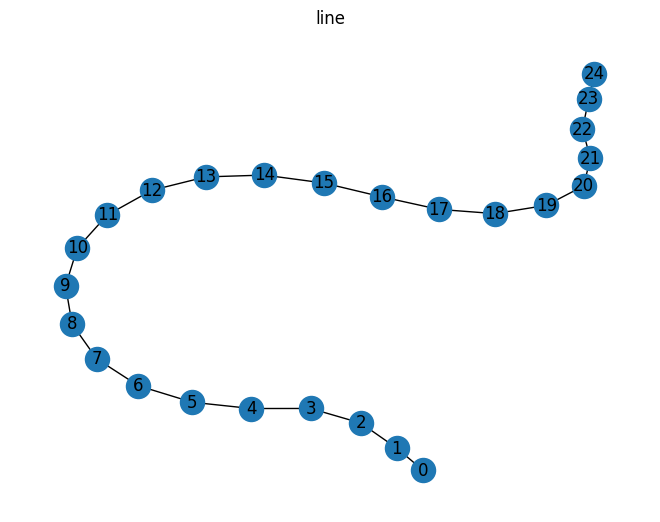
\includegraphics[width=6cm]{images/20_material_methods/path.png}
    \caption{Path oder Line Graph}
    \label{fig:path-graph}
\end{figure}
